\documentclass[12pt]{article}
\usepackage[utf8]{inputenc}
\usepackage[russian]{babel}
\usepackage{graphicx}
\usepackage[none]{hyphenat}
\graphicspath{ {pictures} }
\begin{document}
{\Large\textbf {Отчёт по первому заданию курса "Численное моделирование реагирующих потоков"}\par}
\textit{Выполнил студент 031 группы Александр Казаков}

\section{Численный метод}
Для решения системы нелинейных алгебраических уравнений  $\vec{f}(\vec{u}) = 0$ был использован метод Ньютона. 
На каждой итерации метода искомое решение $\vec{u_k}$ получает приращение $\Delta\vec{u_k}$, рассчитанное из условия:
\begin{eqnarray}
\vec{u_{k+1}} \approx \vec{u_k} + \frac{\partial{\vec{f}}}{\partial{\vec{u}}}\Delta\vec{u_k} = 0
\end{eqnarray}
Для решения полученной СЛАУ использовалась библиотека gsl.
Для лучшей сходимости рассчитанное значение приращения бралось меньшим в два раза (если брать просто решение СЛАУ, 
для данного уравнения метод расходится). 
Было проведено обезразмеривание величин из условия 
\begin{eqnarray}
p' = p/10^6, Q' = Q/10^6, T' = T/10^3, \eta' = \eta,
\end{eqnarray}
что позволило добиться сходимости метода при построении решения для дефлаграции.

\section{Начальное приближение}\label{initAppr}
В качестве начального приближения для решения, соответствующего детонации, использовано
\begin{eqnarray}
p = 10^6p_0, \eta = \eta_0/100, T = 100T_0. 
\end{eqnarray}
В качестве начального приближения для решения, соответствующего дефлаграции, использовано
\begin{eqnarray}
p = p_0/10, \eta = 10\eta_0, T = T_0/10,
\end{eqnarray}
где $p_0 = 10^5Pa, T_0 = 298K$ - нормальные условия, $\eta_0$ рассчитывается с помощью уравнения состояния.

\section{Сходимость}\label{converg}
Для исследования сходимости использовалась обычная евклидова норма - корень из суммы квадратов.
Для случая детонации метод сходится за 48 итераций к значениям, при которых ошибка в $10^{14}$ раз меньше ошибки на начальном приближении.
На рис.\ref{conergencepic} проиллюстрирована сходимость метода при расчёте детонации.
Для случая дефлаграции метод сходится также за 48 итераций.

\begin{figure}[H]
\center{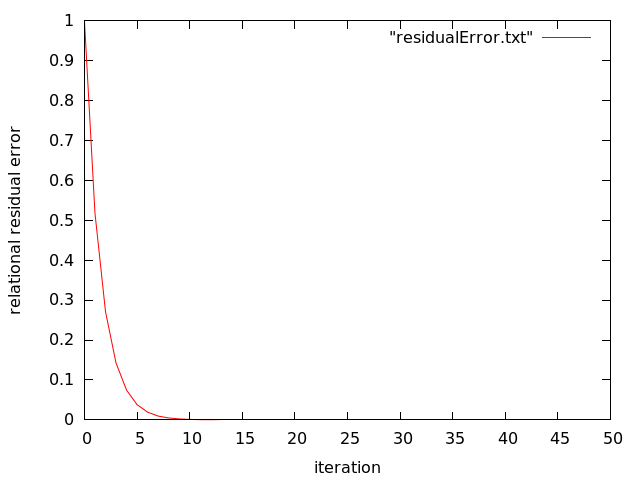
\includegraphics[width=1\linewidth]{pictures/residualError}}
\caption{График зависимости невязки от номера итерации}
\label{conergencepic}
\end{figure}

\section{Результаты}\label{results}
Решение, соответствующее детонации:
\begin{eqnarray}
p = 1.95\cdot10^6 Pa, \rho = 2.04 kg/m^3, T = 3425 K, v = 855 m/s, D = 1973 m/s, \gamma = 1.239. 
\end{eqnarray}
Решение, соответствующее дефлаграции:
\begin{eqnarray}
p = 46\cdot10^3 Pa, \rho = 0.07 kg/m^3, T = 2342 K, v = -783 m/s, D = 51 m/s, \gamma = 1.248. 
\end{eqnarray}

\section{Графики адиабат}\label{hugoniots}
Для построения графиков ударной адиабаты и адиабаты Гюгонио с учётом зависимости $\gamma$ от температуры необходимо
решать нелинейное уравнение на $p$ и $T$ при каждом интересующем фиксированном $\eta$, что и было сделано.
На рис.\ref{hugoniotpic} представлены адиабаты в широком диапазоне значений $\eta$, на рис.\ref{detonationpic} и \ref{deflagrationpic} - 
в более подробном.

\begin{figure}[H]
\center{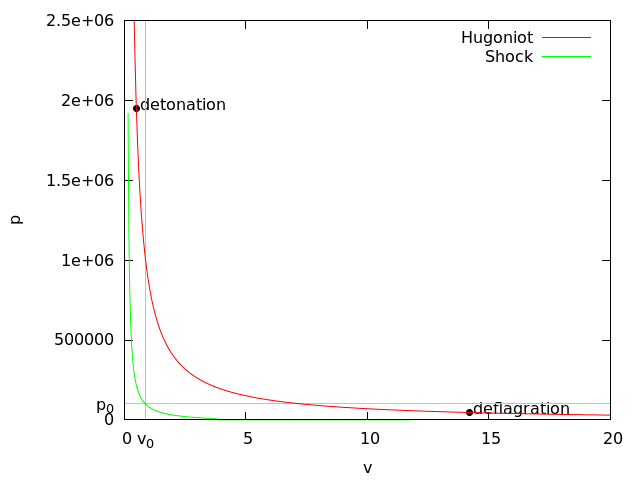
\includegraphics[width=1\linewidth]{pictures/hugoniot}}
\caption{Ударная адиабата и адиабата Гюгонио}
\label{hugoniotpic}
\end{figure}

\begin{figure}[H]
\center{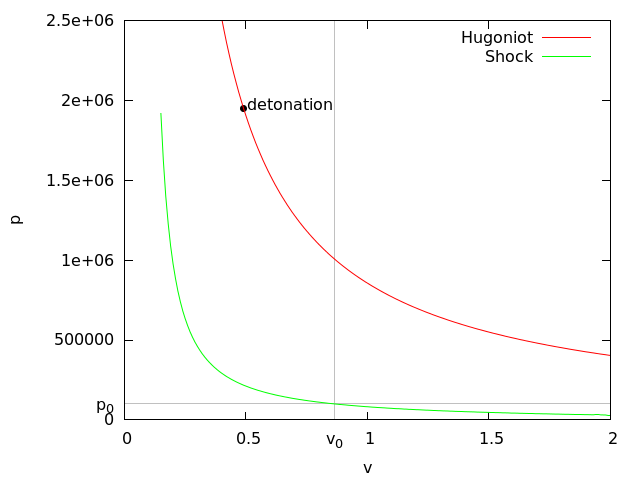
\includegraphics[width=1\linewidth]{pictures/hugoniotDetonation}}
\caption{Ударная адиабата и адиабата Гюгонио}
\label{detonationpic}
\end{figure}

\begin{figure}[H]
\center{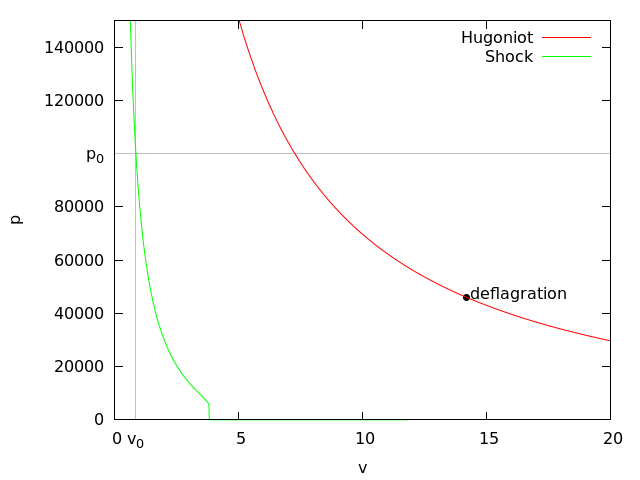
\includegraphics[width=1\linewidth]{pictures/hugoniotDeflagration}}
\caption{Ударная адиабата и адиабата Гюгонио}
\label{deflagrationpic}
\end{figure}

Обрыв ударной адиабаты на рис.\ref{deflagrationpic} происходит из-за того, что при малых значениях $p$ и $T$ метод начинает сходится к нулевым значениям.

\end{document}
